\chapter{Κ-κοντινότερος γείτονας}
\label{appendix:knn}
Ο αλγόριθμος αυτός ανήκει στην κατηγορία των αλγορίθμων  αλγορίθμων βασισμένων σε παραδείγματα, δηλαδή οι προβλέψεις του βασίζονται εξ ολοκλήρου στα παραδείγματα (instances) και δε λαμβάνει χώρα κάποια εκπαίδευση. Οι αλγόριθμοι αυτοί είναι πολύ χρήσιμοι σε εφαρμογές που απαιτούν online μάθηση, επειδή τα δεδομένα έρχονται σειριακά και δεν είναι διαθέσιμα σε ομάδες για εκπαίδευση, όπως σε προβλέψεις μετοχών στο χρηματιστήριο.

Αν φανταστούμε πως τα δεδομένα ζουν σε ένα χώρο ίσων διαστάσεων με το πλήθος των χαρακτηριστικών και διαφοροποιούνται ως προς την κλάση τους, τότε η ταξινόμηση ενός σημείου με άγνωστη κλάση γίνεται ως εξής: βρίσκουμε τους k κοντινότερους γείτονές του και του αναθέτουμε την κλάση της πλειοψηφίας.
\begin{figure}[H]
	\centering			
%	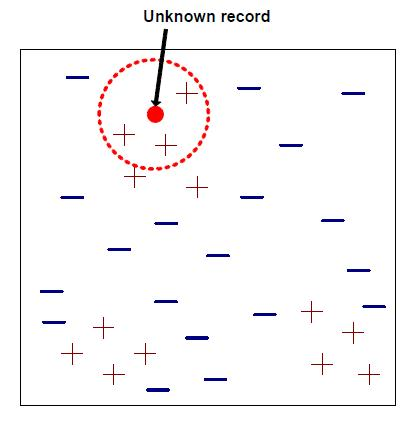
\includegraphics[width=0.6\textwidth, height=6cm]{knn.png}
	\caption[K-NN ταξινομητής]{K-NN ταξινομητής: Το άγνωστο σημείο θα ταξινομηθεί ως θετικό.}
\end{figure}
Μία σημαντική παράμετρος, που εξαρτάται από το πεδίο εφαρμογής, είναι ο τρόπος με τον οποίο υπολογίζεται η απόσταση μεταξύ των σημείων. Διάφορες επιλογές είναι:
\begin{itemize}
	\item \textit{Ευκλείδεια απόσταση.} Πρόκειται για το συνηθέστερο τρόπο υπολογισμού απόστασης και δίνεται από τον τύπο:
	\begin{equation}
	\sqrt[]{\sum_{i=1}^{Κ} (x_i - y_i )^2}
	\end{equation}
	\item \textit{Απόσταση Hamming.} Χρησιμοποιείται για κατηγορικά δεδομένα και κυρίως σε εφαρμογές επεξεργασίας κειμένου. Η απόσταση μεταξύ δύο παραδειγμάτων είναι το άθροισμα της απόστασης μεταξύ των χαρακτηριστικών τους, που ισούται με μηδέν για τα χαρακτηριστικά που συμπίπτουν και ένα για τα υπόλοιπα.
	\item \textit{Απόσταση Manhattan.} Εμπνευσμένη από την οργάνωση του Manhattan σε οικοδομικά τετράγωνα, για τον υπολογισμό της απόστασης μεταξύ δύο σημείων μπορούμε να κινηθούμε μόνο οριζοντίως ή καθέτως. Ορίζεται ως εξής:
	\begin{equation}
	\sum_{i=1}^{Ξ} \abs{x_i - y_i}
	\end{equation}
\end{itemize}

Τέλος, η επιλογή του k οφείλει να γίνει με προσοχή. Αν είναι πολύ μεγάλο υπάρχει ο κίνδυνος κατά την ταξινόμηση να λαμβάνουμε υπόψιν πολύ μακρινά παραδείγματα, ενώ αν είναι πολύ μικρό η ταξινόμηση θα επηρεάζεται εύκολα από ενδεχόμενο θόρυβο στα δεδομένα.
\subsubsection{Συνάρτηση Ακτινικής βάσης }
Η συνάρτηση αυτή σχετίζεται με πολλές έννοιες της μηχανικής μάθησης. Σε αυτό το σημείο θα ορίσουμε το βασικό της μοντέλο και θα δούμε τη λειτουργία της ως τεχνική βασισμένη σε παραδείγματα. 

Η λογική του  μοντέλου αυτού είναι η εξής: η υπόθεση σε ένα σημείο επηρεάζεται από την απόστασή του από κάθε παράδειγμα του σετ εκπαίδευσης. Πιο συγκεκριμένα, η μαθηματική διατύπωση της υπόθεσης, που έχει και τη μορφή του σχήματος που ακολουθεί, είναι η εξής:
\begin{equation}
h(x)= sign( \sum_{n=1}^{N} w_n e^{-\gamma \norm{x - x_n}^2})
\end{equation}
\begin{figure}[H]
	\centering			
%	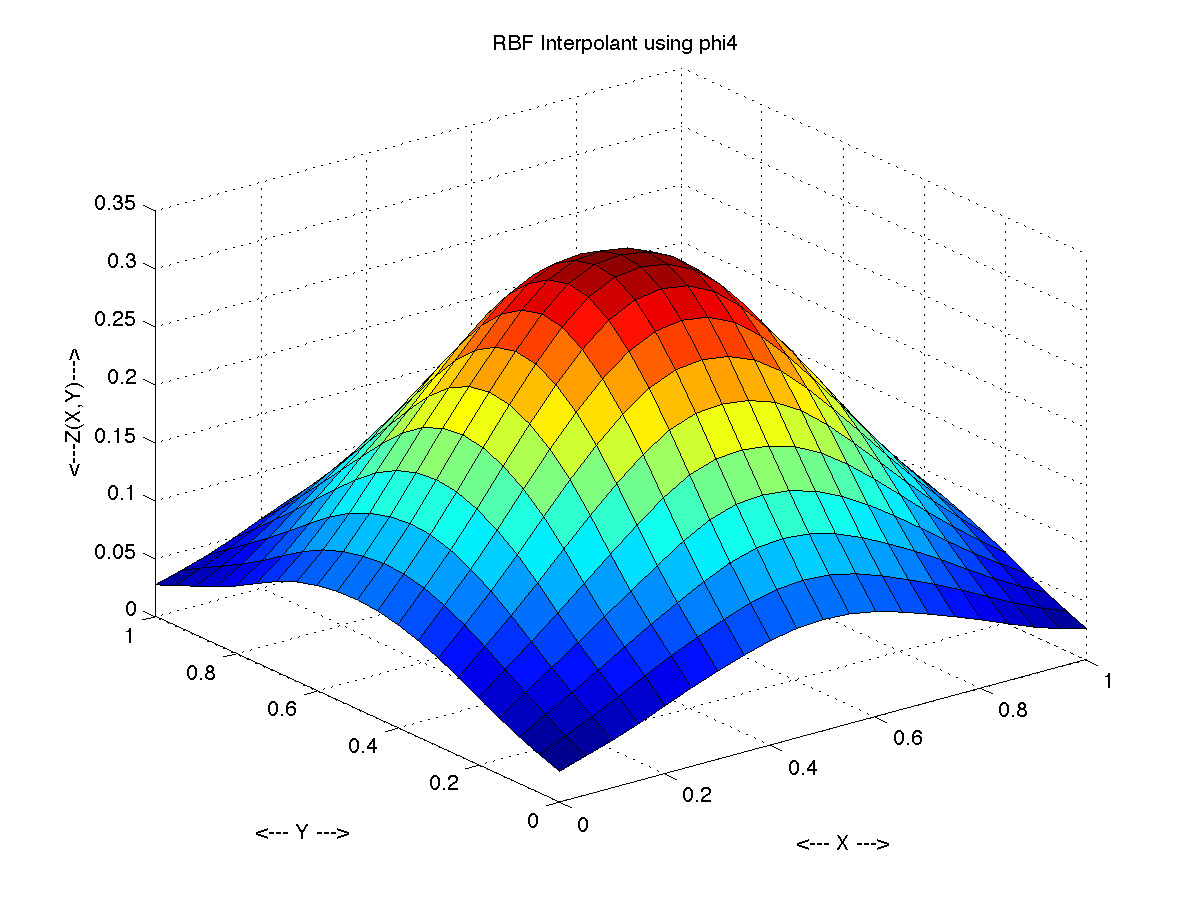
\includegraphics[width=0.6\textwidth]{rbf.png}
	\caption[Radial Basis συνάρτηση με γκαουσιανή βάση]{Radial Basis συνάρτηση με γκαουσιανή βάση.}
\end{figure}
Η επιλογή της βέλτιστης υπόθεσής έγκειται σε αυτήν που προβλέπει σωστά όλα τα παραδείγματα του σετ εκπαίδευσης. Αν και συνήθως προσπαθούμε να ελαχιστοποιήσουμε το σφάλμα, εδώ είμαστε σίγουροι πως θα καταφέρουμε να το μηδενίσουμε, καθώς το μοντέλο μας έχει στη διάθεση του πάρα πολλές παραμέτρους (όσα είναι και τα παραδείγματα). Επομένως το πρόβλημα βελτιστοποίησης ορίζεται ως:
\begin{equation}
E_{in}=0 \rightarrow  \sum_{n=1}^{N} w_n e^{-\gamma \norm{x_n - x_m}^2}= y_n  \forall n \in D_N 
\end{equation}
όπου $E_{in}$ είναι το σφάλμα στα παραδείγματα εκπαίδευσης και $D_N$ το σετ εκπαίδευσης. 

Ο παραπάνω τύπος δίνει ένα σύστημα Ν γραμμικών εξισώσεων με Ν αγνώστους που διατυπώνεται εύκολα ως εξής:
\[
\underbrace{
	\begin{bmatrix}
	e^{-\gamma \norm{x_1 - x_1}^2}  & \dots  &  e^{-\gamma \norm{x_1 - x_N}^2} \\
	e^{-\gamma \norm{x_2 - x_1}^2}  & \dots  &  e^{-\gamma \norm{x_2 - x_N}^2} \\
	\vdots  & \vdots & \vdots \\
	e^{-\gamma \norm{x_N - x_1}^2}  & \dots  &  e^{-\gamma \norm{x_N - x_N}^2} \\
	\end{bmatrix}}_{  \Phi}
\underbrace{
	\begin{bmatrix}
	w_{1}       \\
	w_{2}        \\
	\vdots        \\
	w_{N}
	\end{bmatrix}}_{W}
=
\underbrace{
	\begin{bmatrix}
	y_{1}       \\
	y_{2}        \\
	\vdots        \\
	y_{N}
	\end{bmatrix}}_{Y}
\]

Η λύση αυτού του συστήματος δίνεται από τον τύπο:
\begin{equation}
w=\inv{\Phi} y
\end{equation}

όπου ο πίνακας $\Phi$ πρέπει να είναι αντιστρέψιμος

\paragraph{Επίδραση της μεταβλητής γ} Η μεταβλητή αυτή ορίζει πόσο απλωμένη είναι η καμπάνα γύρω από κάθε σημείο του σετ εκπαίδευσης και άρα πόσο επίδραση έχει αυτό στη γειτονιά του.
\begin{figure}[H]
	\centering
	\begin{minipage}{.5\textwidth}
		\centering
%		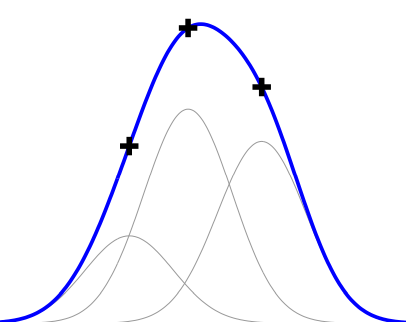
\includegraphics[width=0.8\linewidth, height=0.15\textheight]{smallg.png}
		\caption[RBF με μικρό γ]{RBF με μικρό γ}		
	\end{minipage}%
	\begin{minipage}{0.5\textwidth}
		\centering
%		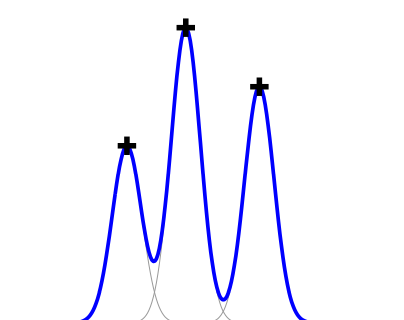
\includegraphics[width=0.8\linewidth, height=0.15\textheight]{big.png}
		\caption[RBF με μεγάλο γ]{RBF με μεγάλο γ}		
	\end{minipage}
\end{figure}
\paragraph{H συνάρτηση RBF ως μοντέλο βασισμένο σε παραδείγματα.} Όπως είδαμε η ταξινόμηση ενός σημείου εξαρτάται από την απόστασή του από τα υπόλοιπα του σετ εκπαίδευσης, τεχνική που παραπέμπει άμεσα στη λογική της κατηγοριοποίησης με βάση τα παραδείγματα. Μέχρι τώρα έχουμε θεωρήσει ως συνάρτηση βάσης την γκαουσιανή, αν όμως τοποθετήσουμε έναν απλό κύλινδρο γύρω από κάθε σημείο, η τεχνική αυτή ταυτίζεται με το μοντέλο k-NN.
\paragraph{Επιλογή Κ κέντρων.} Η χρήση τόσων παραμέτρων όσων είναι και τα στοιχεία του σετ εκπαίδευσης κάνει τη διαδικασία της εκπαίδευσης χρονοβόρα και ενέχει κινδύνους υπερπροσαρμογής. Συνήθως λοιπόν χρησιμοποιούμε μια τροποποίηση της τεχνικής που έχουμε περιγράψει, όπου αντί να υπολογίζουμε την απόσταση από όλα τα σημεία, επιλέγουμε Κ αντιπροσωπευτικά σημεία του χώρου και τους αναθέτουμε κάποια από τα σημεία του σετ εκπαίδευσης. Έτσι, σχηματίζονται ομάδες σημείων που αντιπροσωπεύονται από το κέντρο τους και απαιτείται πλέον ο καθορισμός Κ και όχι Ν παραμέτρων.

Πλέον η υπόθεση δίνεται από τον τύπο:
\begin{equation}
h(x)= sign( \sum_{k=1}^{K} w_n e^{-\gamma \norm{x - \mu_k}^2})
\end{equation}

όπου $\mu_k$ είναι το κέντρο μιας ομάδας. Η επιλογή των βαρών $w_n$ είναι παρόμοια: έχω Ν εξισώσεις και Κ παραμέτρους, οπότε το σύστημα λύνεται με τη χρήση του ψευδοαντίστροφου πίνακα:
\begin{equation}
w= \inv{\Phi^T \Phi} \Phi^T y
\end{equation}
\fbox{\begin{minipage}{\textwidth}
		\begin{center}
			Επίλυση υπερορισμένων συστημάτων με χρήση ψευδοαντίστροφου
		\end{center} 
		Ένα γραμμικό σύστημα $y=A x$ χαρακτηρίζεται ως υπερορισμένο όταν έχει περισσότερες εξισώσεις από αγνώστους. Σε αυτή τη περίπτωση ο πίνακας Α είναι μη τετραγωνικός και επομένως μη αντιστρέψιμος, οπότε η λύση δεν μπορεί να δοθεί ως συνήθως από $x=\inv{A} y$. Μία συνήθης λύση είναι η χρήση του ψευδοαντίστροφου Moore-Penrose, που ορίζεται ως $ A\ssymbol{2}\ = \inv{(A^T A)} A^T$, ώστε να ισχύει $A\ssymbol{2}\ Α=Ι$, αλλά όχι $Α A\ssymbol{2}\=Ι$. Τότε, ο πολλαπλασιασμός και των δύο μερών της εξίσωσης με $ A\ssymbol{2}\ $ δεν εγγυάται ισότητα, αλλά προσέγγιση ελαχίστων τετραγώνων και η λύση είναι $x \approx A\ssymbol{2}\ y $
	\end{minipage}}
	
	Το νέο πρόβλημα που αναδύεται είναι αυτό της επιλογής των βέλτιστων $\mu_k$. Το πρόβλημα αυτό επιλύεται με την τεχνική της k-means ομαδοποίησης και διατυπώνεται ως εξής: Πρέπει να διαχωρίσουμε τα σημεία $x_1,..., x_n$ σε k ομάδες $S_1,...,S_k$, ώστε να ελαχιστοποιήσουμε το μέγεθος:
	\begin{equation}
\sum_{k=1}^{K} \sum_{x_n \in S_k} \norm{x_n - \mu_k}^2
\end{equation}
	που δίνει το άθροισμα των αποστάσεων κάθε σημείου από το κέντρο της ομάδας στην οποία ανήκει.
	
	Η λύση του δίνεται από τον αλγόριθμο του Lloyd, που εντοπίζει ένα τοπικό ελάχιστο επαναληπτικά σπάζοντας τη διαδικασία σε δύο ανεξάρτητα στάδια:
	\begin{itemize}
		\item \textit{υπολογισμός κέντρων.} Δεδομένων των ομάδων, το κέντρο κάθε ομάδας παίρνει την μέση τιμή των σημείων που της ανήκουν.
		\item \textit{υπολογισμός ομάδων.} Για κάθε σημείο του σετ εκπαίδευσης υπολογίζουμε την απόστασή του από το κέντρο κάθε ομάδας και το αναθέτουμε στην κοντινότερη ομάδα.
	\end{itemize}
	
	Η διαδικασία επαναλαμβάνεται μέχρι να συγκλίνουμε σε μια ομαδοποίηση των σημείων, δηλαδή οι ομάδες να μη μεταβάλλονται σε μια επανάληψη του αλγορίθμου.